\chapter{Collapsed Variational Approximation}

\setlength{\parindent}{0pt}

\section{Introduction}

Bayesian model selection is a powerful set of techniques for model selection. These techniques are especially
useful in problems of high-dimension, such as bioinformatics problems where the model space is complex and the
optimal model is difficult for statisticians to manually specify. But Bayesian model selection is
computationally expensive, and prone to getting stuck in local minima if the posterior likelihood is multi-
modal. This issue is particularly acute if the spike-and-slab prior, popular for Bayesian model
selection, is used. We seek to address both problems by proposing a population non-parametric Variational
Bayes approximation algorithm - a population-based optimisation strategy. Maintaining a population of models
allows the posterior distribution to be explored more thoroughly, finding multiple maxima. The variational
approximation's lower bound includes an entropy term which ensures diversity in the population by penalising
similarity,  having the particles in the population repel each other. This ensures the high probability
regions of the posterior distribution is thoroughly explored, which better reflects model selection
uncertainty.

In this chapter, we focus on the important case of model selection for normal linear models which
are slightly altered from those introduced in Section \ref{sec:model} to incorporate a zero-centred normal
prior on $\alpha$ with variance $g \sigma^2$. This allows shrinkage of the intercept as well as the
non-intercept regression co-efficients, driven by data.

\cite{Mitchell1988} initially proposed the spike-and-slab prior distribution on regression co-efficients not
currently included in the model -- which places a mixture of a point mass 'spike' at $0$ and a diffuse uniform
distribution 'slab' elsewhere. The approach was further developed by \cite{Madigan1994} to incorporate an
alternative Bayesian approach that takes full account of the true model uncertainty by averaging over a small
subset of models, and an efficient search algorithm for finding these models. \cite{George1997} investigated
computational methods for posterior evaluation and exploration in this setting, and using Gray Code sequencing
and Markov Chain Monte Carlo to explore the model space in moderate and large-sized problems respectively.
More recently, \cite{Ishwaran2005} developed a rescaled spike-and-slab model which improves effective variable
selection in terms of risk misclassification by using selective shrinkage.

% We further extend this approach, by
% using the Cake variant of the spike-and-slab prior for model selection \cite{OrmerodEtal2017}, as it avoids
% the Lindley and Bartlett paradoxes \cite{Lindley1957}, \cite{Bartlett1957}.

Existing approaches to the problem of model selection focus upon finding a single best model as quickly as
possible, using the least computational effort (\cite{You2014}, \cite{Rockova2014}). Exploring the model space
using only one model at a time will provide a misleading view of the uncertainty in the posterior, as it is
typically highly multimodal.

Many computational schemes for Bayesian model selection exist, using Monte Carlo Markov Chains techniques to
compute the posterior distribution of $\vgamma$. However, these schemes are both computationally intensive and
can become trapped in local maxima of the posterior distribution if the distribution is high-dimensional and
multi-modal, as is the case with popular choices of prior for Bayesian model selection problems, such as
spike-and-slab priors. The difficulty of becoming trapped in local maxima can be partially mitigated by using
population-based MCMC schemes such as Jasra et al. 2007, Bottolo and Richardson 2010, Hans et al 2007, Liang
and Wong 2000. However, this increases the computational cost of sampling from the posterior distributions
still further, especially in high-dimensional problems.

\cite{Rockova2016} introduced the notion of Particle EM. Rather than searching for a single optimal model,
Particle EM instead maintains a population of models (particles). This allows the algorithm to explore more of
the posterior model space, gaining a better estimate of the variation of the model space than an algorithm
involving only a single model. It also allows the particles to ``interact'', searching for the essential
posterior modes together. In Particle EM, this is done by incorporating an ``entropy term'' in the variational
lower bound, which ensures diversity amongst the models in the population, preventing all particles from
simply seeking the global posterior modes. The algorithm is determininistic.

We build upon this work by proposing a fixed-form parametric Variational Bayes approximation of $\vgamma$. We
adopt a prior structure incorporating the Cake prior for variable selection, which avoids the Lindley and
Bartlett's paradoxes. The difficulties in implementing practical Bayesian model selection schemes have been
noted in \cite{Chipman2014}. As our marginal likelihood expression is a function only of $n$, $p_\vgamma$ and
$R^2_\vgamma$, our model selection algorithm can be executed efficiently using rank-one updates and downdates
to compute $R^2_{\vgamma^*}$ for each of the models $\vgamma^*$ that we consider. To ensure uniqueness of the
$K$ models in the population, before a new candidate model with a covariate added or removed is considered,
the population of existing models is checked to see if it already exists in the population. If so, the
addition or removal of the covariate is skipped and the next candidate model considered.

% Collapsed Variational Bayes
% Collapsed Variational Bayes approaches have proved useful in Bayesian nonparametric settings such as Latent
% Dirichlet Allocation \cite{Teh2007}
Our variational approximation is a fixed form parametric approximation which places a weight on each covariate
\[
	q(\vgamma) = \sum_{k=1}^K w_k \I(\vgamma_k)
\]

% Population-based MCMC approaches

Our main contributions are:

\begin{enumerate}
	\item Our algorithm searches over the binary strings $\vgamma$ directly, as the estimates of $\vbeta$ are available 
	in closed form once $\vgamma$ is known.

	\item We make use of a population--based optimisation scheme to search the model space. We take advantage of the
	population of solutions by incorporating a penalty for lack of entropy, which ensures diversity in the
	population of solutions.

	\item The entire trajectory of particles gives far more information about variable selection than a single
	snapshot of the final best decision.

	\item Our model can incorporate different hyperpriors on $g$ and $\vgamma$. Using a hyperprior on $g$
				avoids Lindley's paradox and Bartlett's paradox, the model selection paradoxes which arise when a
				fixed choice of $g$ is made.
\end{enumerate}

This article is organised as follows. In Section 2, we detail the derivation of our approximation and fitting
algorithms. In Section 3, we discuss computational issues with implementing our algorithm efficiently. In
Section 4, we present the results of our numerical experiments. In Section 5, we present our conclusions and
discuss our results.

% \section{Method}

% \subsection{Posterior distributions of $g$-priors in terms of special functions}
% % Things we derived


% \subsubsection{Calculating $p(\vy | \vgamma)$}
% We want to calculate $p(\vy | \vgamma)$ so that we can calculate $p(\vgamma | \vy)$ using Bayes' Rule 
% allowing us to rank models against one another and choose which amongst many candidate models is best.
% To do this, we need to calculate
% $$p(\vy | \vgamma) = \int p(\vy | \alpha, \vbeta, \sigma^2, \vgamma) p(\alpha) p(\vbeta | g, \vgamma) p(\sigma^2) p(g) d \alpha d \vbeta d \sigma^2 d g.$$
% We choose our priors so that this integral is tractable, with help from \cite{Gradshteyn1988}.
% The marginal likelihoods obtained from this integral behave like BIC.

% We found the following closed form expressions. Include derivations in the appendices.
% \small
% \begin{itemize}
% 	\item Liang et al. 2008 hyper-$g$ prior \cite{Liang2008}
% 		$p(\vy | \vgamma) = \frac{K(n) (a - 2)}{p_\vgamma + a  - 2} {}_2 F_1 \left( \frac{n-1}{2}, 1; \frac{p_\vgamma + a}{2}; R_\vgamma^2 \right)$
% 	\item Liang et al. 2008 hyper-$g/n$ prior \cite{Liang2008}
% 		$p(\vy | \vgamma) = \frac{K(n) (a - 2)}{n (p_\vgamma + a  - 2)} F_1 \left( 1, \frac{a}{2}, \frac{n-1}{2}; \frac{p_\vgamma + a}{2}; 1 - \frac{1}{n}, R_\vgamma^2 \right)$
% \end{itemize}
% These expressions are numerically stable to evaluate.

% We want to be able to calculate the marginal likelihood of the data given $\vgamma$, so that we can
% calculate the posterior probability of $\vgamma$ and rank models against one another. To do this, we
% need to calculate the following integral.
% We choose our priors so that this integral is tractable, with help from the book Table of Integrals and
% Series by Gradshteyn. The marginal likelihoods behave like BIC.
% We found closed form expressions for the marginal likelihood for the hyper-$g$ and hyper-$g/n$ priors.

% \subsubsection{Calculating $p(\vy | \vgamma)$ for Bayarri's robust prior}
% \begin{itemize}
% 	\item Bayarri calculated the marginal likelihood given $\vgamma$ for the Robust Bayarri prior
% 	 	in \cite{Bayarri2012} 
% 		\tiny
% 		$p(\vy | \vgamma) = K(n) \left(\frac{n + 1}{1 + p_\vgamma}\right)^{-p_\vgamma/2} \frac{(1 - R^2_\vgamma)^{-(n-1)/2}}{p_\vgamma + 1} {}_2 F_1 \left[ \frac{n-1}{2}, \frac{p_\vgamma+1}{2}; \frac{p_\vgamma + 3}{2}; \frac{[1 - 1/(1 - R^2_\vgamma)](p_\vgamma + 1)}{1 + n} \right]$.
% 	\small
% 	\item But this expression is not numerically well-behaved, because the second argument of the
% 				${}_2 F_1$ function is greater than $1$.
% 	\item Using a trick that's available when ${}_2 F_1(., 1; .; .)$ ... is numerically
% 				well-behaved, we derived the new expression
% 		\tiny
% 		$p(\vy | \vgamma) = K(n) \left(\frac{n + 1}{1 + p_\vgamma}\right)^{(n-p_\vgamma-1)/2} \frac{[1 + L (1 - R^2_\vgamma)]^{-(n-1)/2}}{p_\vgamma + 1} {}_2 F_1 \left[ \frac{n-1}{2}, 1; \frac{p_\vgamma + 3}{2}; 
% 		\frac{R^2_\vgamma}{1 + L(1 - R^2_\vgamma)} \right]$ \\
% 		\small
% 		where $L = (1 + n)/(1 + p_\vgamma) - 1$.
% \end{itemize}

% Bayarri calculated the marginal likelihood given $\vgamma$ for the Robust Bayarri prior.
% But this expression is not numerically well-behaved.
% We used Euler's transformation and properties of the hypergeometric function to derive a new,
% numerically stable function.


\section{Bayesian linear model averaging}

We will start with the following linear model for predicting $\vy$ with design matrix $\mX$ via
\begin{equation}\label{eq:linearModel}
\ds \vy | \alpha, \vbeta, \sigma^2 \sim N_n(\vone_n\alpha + \mX \vbeta, \sigma^2 \mI_n),
\end{equation} 


\noindent where 
$\vy = (y_1,\ldots,y_n)^T$ is a response vector of length $n$, $\mX$ is an $n \times p$ matrix 
of covariates,
$\alpha$ is the model intercept, $\vbeta$ is a coefficient vector of length $p$, 
$\sigma^2$ is the residual variance, and $\mI_n$ is the $n \times n$ identity matrix. 
We standardize $\vy$ and $\mX$ 
so that $\overline{y} = 0$, 
$\|\vy\|^2 = \vy^T\vy = n$, $\overline{\mX}_j = 0$,  and $\|\mX_j\|^2 = n$ where $\mX_j$ is the $j$th 
column of $\mX$ to simplify algebra and so that predictors are in the same scale.

\subsection{Prior structure on the linear model parameters} 

We will adopt a priors structure for $\alpha$, $\vbeta$ and $\sigma^2$ conditional
a model  vector $\vgamma\in \{0, 1\}^p$ and a prior hyperparameter $g$  given by
\begin{equation}
\label{eq:priorStructure}
\begin{array}{c}
\ds p(\alpha) \propto 1,  
\qquad 
\vbeta_\vgamma | \sigma^2, g, \vgamma \sim N_p(\vzero, g \sigma^2 (\mX_\vgamma^T \mX_\vgamma)^{-1}), \\[1ex]
\ds p(\vbeta_{-\vgamma}|\vgamma) = \prod_{j=1}^p \delta(\beta_j;0)^{1-\gamma_j}
\quad \text{ and }  \quad 
\ds p(\sigma^2) \propto (\sigma^2)^{-1} I(\sigma^2 > 0),                      
\end{array}
\end{equation} 

\noindent where $\mX_\vgamma$ denotes the design matrix formed by including only the 
$j$th column of $\mX$ when $\gamma_j = 1$,
where $\delta(x;a)$ is the Dirac delta function with location $a$.  
The prior on $\vbeta_\vgamma$ is Zellner's $g$-prior \citep[see for example,][]{Zellner1986} with prior 
hyperparameter $g$. This family of priors for a Gaussian regression model where the prior covariance 
matrix of $\vbeta_\vgamma$ is taken to be a multiple of $g$ with the Fisher information matrix for $\vbeta$, and makes the marginal likelihood of the model scale-invariant.
The prior on $\vbeta_{-\vgamma}$ in (\ref{eq:priorStructure}) is the spike in
in what is referred to as a spike and slab prior where the prior on $\vbeta_{\vgamma}$ is assumed to be flat (the slab). 
The above structure implies 
that $p(\vbeta_{-\vgamma}|\vy)$ is a point mass at $\vzero$
and leads to
algebraic and computational simplifications for components of $\vbeta$ when elements of $\vgamma$ equal 0.
Thus, $\gamma_j=0$ is equivalent to excluding the corresponding predictor $\mX_j$ from the model.

Integrating out $\alpha$, $\vbeta$, and $\sigma^2$ from $p(\vy,\alpha,\vbeta,\sigma^2|g,\vgamma)$ we
obtain
\begin{equation}\label{eq:yGivenG}
\begin{array}{rl}
\ds p(\vy|g,\vgamma)
%& \ds = \int \exp\left[
%- \tfrac{n-1}{2}\log(2\pi) 
%- \tfrac{1}{2}\log(n)
%- \tfrac{p}{2}\log(1 + g)
%- \left( \tfrac{n-1}{2} + 1\right)\log(\sigma^2) 
%- \left( \tfrac{n}{2} \tfrac{1 + g(1-R^2)}{1 + g} \right)\sigma^{-2} 
%\right]  d\sigma^2
%\\
%& 
\ds = K(n)
(1 + g)^{(n - p_\vgamma - 1)/2}(1 + g (1 - R_\vgamma^2))^{-(n-1)/2},
\end{array} 
\end{equation}

\noindent where $K(n) = [\Gamma( (n-1)/2 )]/[\sqrt{n}(n\pi)^{(n-1)/2}]$, 
$R_\vgamma^2 = \vy^T\mX_\vgamma^T(\mX_\vgamma^T\mX_\vgamma)^{-1}\mX_\vgamma^T\vy/n$ is 
the usual R-squared statistic for model $\vgamma$, and $p_\vgamma$ is the number
of variables in the model $\vgamma$.

% Justify choice of prior

\cite{Liang2008} considered several approaches to specifying $g$, including letting $g$ diverge,
setting $g$ to a constant, choosing $g$ adaptively via a local or global empirical Bayes procedure,
and placing a hyperprior should  on $g$. They argued that for desirable inferential properties that a  hyperprior 
should be placed on $g$.
For a given hyperprior on $g$ we define the (null based) Bayes factor for a model $\vgamma$ given by
$$
\ds \mbox{BF}(\vgamma) = \frac{p(\vy|\vgamma)}{p(\vy|\vzero)}.
$$

\noindent Note that the Bayes factor is a statistic commonly used in Bayesian hypothesis testing
\citep{Raftery1997,OrmerodEtal2017}.
Values of BF greater than 1 lead to preferring the model $\vgamma$ and values
less than 1 lead to preferring the null model $\vgamma=\vzero$, i.e., the model containing only
the intercept. Note that
when $\vgamma = \vzero$, i.e., the null model, then $p_\vgamma = 0$, and
$R_\vgamma^2 = 0$ leading to the simplification $p(\vy|g,\vzero) = K(n)$
for all $g$. Hence, $p(\vy|\vzero) = K(n)$ provided the hyperprior on $g$ is a proper density.  

\subsection{Hyperpriors on $g$}

Recently, Greenaway \& Ormerod (2018) examined several hyperpriors on $g$ considered in the literature.
These included the hyper-$g$ and hyper-$g/n$ priors of \cite{Liang2008}, the beta-prime prior of \cite{Maruyama2011}, 
the robust prior of \cite{Bayarri2012}, and the cake prior of \cite{OrmerodEtal2017}. They showed how 
all of these, except for the hyper-$g/n$ priors can be evaluated an efficient, accurate and 
numerically stable manner. 
We summarise their results in the list below.
\begin{itemize}
	\item The {\bf hyper-$g$} prior of \cite{Liang2008} given by
	$p_{g}(g) = \frac{a - 2}{2}(1 + g)^{-a/2}$,
	for $a>2$ and $g>0$ leads to
	\begin{equation}\label{eq:hyperGmarginal2}
	\ds \mbox{BF}_g(\vgamma)
	=  
	\frac{a - 2}{2 R_\vgamma^2(1 - R_\vgamma^2)} 
	\frac{\mbox{pbeta}\left(R_\vgamma^2,\tfrac{p_\vgamma + a - 2}{2},\tfrac{n-p_\vgamma - a+1}{2}\right)}{
		\mbox{dbeta}\left(R_\vgamma^2,\tfrac{p_\vgamma + a - 2}{2},\tfrac{n-p_\vgamma - a+1}{2}\right)},
	\end{equation}
	
	where $\mbox{pbeta}(x;a,b)$ and $\mbox{dbeta}(x;a,b)$  are the cdf and pdf of the beta 
		distribution respectively. The value $a=3$ is typically used. Note that \cite{Liang2008} derived an equivalent expression in terms of the Gaussian hypergeometric function ${}_2 F_{1}(\cdot,\cdot;\cdot,\cdot;\cdot)$. The above expression is numerically easier to work with.
		
		\item The {\bf robust} hyperprior for $g$ proposed by \cite{Bayarri2012} is designed to have several nice theoretical
		properties outlined there. Using their default parameter
		choices, the hyperprior 
		on $g$ used by \cite{Bayarri2012} corresponds to 
		$p_{{rob}}(g) = \tfrac{1}{2}r^{1/2} (1 + g)^{-3/2} I(g>L)$  where $L = r - 1$ and $r = (1 + n)/(1 + p_\vgamma)$. 
		Letting $\widetilde{R}_\vgamma^2 = R_\vgamma^2/(1 + L\widehat{\sigma}_\vgamma^2)$
		the Bayes factor can be written as
		\begin{equation}\label{eq:yGivenGammaRobust2}
		%\begin{array}{rl}
		\ds \mbox{BF}_{{rob}}(\vgamma)
		%& \ds = \left( \frac{1 + n}{1 + p_\vgamma} \right)^{(n - p_\vgamma - 1)/2} \frac{\left( 1 + L\widehat{\sigma}_\vgamma^2 \right)^{-(n - 1)/2}}{1 + p_\vgamma}
		%{}_2F_1\left(  
		%\frac{n-1}{2}, 1; \frac{p_\vgamma+3}{2}; \frac{1 - \widehat{\sigma}_\vgamma^2}{1 + L\widehat{\sigma}_\vgamma^2}
		% \right)
		%\\
		%& \ds 
		= r^{(n - p_\vgamma - 1)/2} \frac{\left( 1 + L\widehat{\sigma}_\vgamma^2 \right)^{-(n - 1)/2}}{2 \widetilde{R}_\vgamma^2(1 - \widetilde{R}_\vgamma^2)} 
		\frac{
			\mbox{pbeta}\left( 
			\widetilde{R}_\vgamma^2,
			\frac{p_\vgamma +1}{2},
			\frac{n - p_\vgamma - 2}{2} 
			\right)
		}{
			\mbox{dbeta}\left( 
			\widetilde{R}_\vgamma^2,
			\frac{p_\vgamma +1}{2},
			\frac{n - p_\vgamma - 2}{2} 
			\right)
		}.
		%\end{array}
		\end{equation}
		
		\noindent Again, \cite{Bayarri2012} derived an equivalent expression in terms of ${}_2 F_1$, however
		(\ref{eq:yGivenGammaRobust2}) is numerically easier to work with.
 
		
	\item The {\bf beta-prime} hyperprior on $g$ employed by \cite{Maruyama2011} is given by
	$p_{bp}(g) = g^{b}(1 + g)^{-(a+b+2)}/\mbox{Beta}(a+1,b+1)$,
	where $g>0$, $a>-1$ and $b>-1$, i.e.,
	$g\sim \mbox{Beta-Prime}(b+1,a+1)$ using the typical parametrization of 
	the beta-prime distribution \citep{Johnson1995}. When	 $b = (n - p_\vgamma - 5)/2 - a$ 
	the corresponding Bayes factor simplifies to
	\begin{equation}\label{eq:marginalLikelihoodBetaPrime}
	\begin{array}{rl}
	\ds \mbox{BF}_{bp}(\vgamma) 
	%& \ds =
	%\frac{K(n)}{\mbox{Beta}(a+1,b+1)}
	%\int_0^\infty g^{b} \left[ 1 + g(1-R^2) \right]^{-(n-1)/2}  
	%dg
	%\\ [2ex]
	& \ds 
	=   
	\frac{\mbox{Beta}(p/2 + a + 1,b + 1)}{\mbox{Beta}(a+1,b+1)} (1-R_\vgamma^2)^{-(b + 1)}
	%\\ [2ex]
	%& \ds = \widetilde{K}(n,a)
	%
	%\Gamma(p/2 + a + 1)\Gamma(a + b + 2)
	%(\widehat{\sigma}^2)^{-(b + 1)}
	\end{array}
	\end{equation}	
	
	\noindent where $\mbox{Beta}(u,v) = \Gamma(u)\Gamma(v)/\Gamma(u+v)$ is the beta function.
	The default value for $a$ chosen by 
	\cite{Maruyama2011} is $a = -3/4$. Note that the prior used in \cite{Maruyama2011} for
	$\vbeta_\vgamma$ is different than from what we use here. Greenaway \& Ormerod (2018) discuss
	these differences and justify our choice.
	
	\item The {\bf cake} prior of \cite{OrmerodEtal2017} 
	departs from the prior structure (\ref{eq:priorStructure}) and instead uses
	\begin{equation}\label{eq:proirs2}
	\begin{array}{c}
	\ds \alpha|\sigma^2,g \sim N(0,g\sigma^2), \quad 
	\ds \vbeta_\vgamma|\sigma^2,g \sim N\left( \vzero,g\sigma^2\left( \tfrac{1}{n}\mX_\vgamma^T\mX_\vgamma\right)^{-1}\right)
	\\ \mbox{and} \quad
	p(g|\vgamma_j) = \delta(g; h^{1/(1 + p_\vgamma)})
	\end{array} 
	\end{equation}
	
	\noindent where $h$ is a common prior hyperparameter for all models. This is slightly
	different from (\ref{eq:priorStructure}). The log   Bayes factor
	as a function of $h$ 
	for model $\vgamma$ is of the form
	$$
	\begin{array}{rl}
	\ds \log\mbox{BF}(\vgamma;h)
	=
	-\tfrac{n}{2}\log\left( 1 - \tfrac{h^{1/(1+p_\vgamma)}}{1+h^{1/(1+p_\vgamma)}} R_\vgamma^2 \right) 
	- \tfrac{p_\vgamma}{2}\log\left(n + h^{-1/(1+p_\vgamma)} \right).
	\end{array}
	$$
	
	\noindent Taking $h\to\infty$ we obtain a null based Bayes factor approaches
	\begin{equation}\label{eq:marginalLikelihoodCake}
	\ds \mbox{BF}_{\mbox{\scriptsize cake}}(\vgamma)
	=
	\exp\left[ \,
	-\tfrac{n}{2}\log\left( 1 - R_\vgamma^2 \right) 
	- \tfrac{p_\vgamma}{2}\log\left(n \right) \,
	\right] = \exp\left[ \, -\tfrac{1}{2}\mbox{BIC}(\vgamma) \,\right]
	\end{equation}
	
	\noindent where $\mbox{BIC}(\vgamma) = n\log\left( 1 - R_\vgamma^2 \right) + p_\vgamma \log(n)$ is the Bayesian 
	Information of \cite{Schwarz1978} modulo constants which only depend on the sample size (and so are common to all models). 
\end{itemize}

\noindent All of the above Bayes factors can be evaluated on the log-scale using standard software avoiding numerical overflow and stability issues.
All of the above hyerpriors on $g$ lead to model selection consistency under mild assumptions, except for 
the hyper-$g$ prior which is only model selection consistent when the true model is
not the null model. 

\subsection{Prior on the model space/size}

The last ingredient to a fully Bayesian model specification is the prior on $\vgamma$,
sometimes referred to as a prior on the model space, or model size.
As the dimension of the problem increases the choice of model prior becomes
increasingly important. The two most commonly 
used priors are to use a uniform prior on the model space
and the beta-binomial probability on the model size.
The choices of prior for the model space/size has been discussed
in detail by \cite{scott2010} and are also discussed in \cite{castillo2015}.

A uniform prior on the space of all models puts an equal prior probability on each model, i.e., 
$$
\ds p(\vgamma) = 2^{-p} \qquad \mbox{for all $\vgamma\in\{0,1\}^p$},
$$

\noindent which is equivalent to $p(\gamma_j) = 1/2$, $1\le j\le p$. While this model prior
has the appeal of being flat or uninformative, it is a poor  choice as a default prior for high dimensional 
problems. \cite{scott2010} state that this model prior provides no multiplicity control in a multiple 
testing setting, and uses an a priori model size of $p/2$ with a standard deviation of $\sqrt{p}/2$ 
leading to an a priori large fraction of covariates being included when $p$ is large. We have found that this choice
of prior works poorly on high dimensional problems in practice.

The beta-binomial prior on the model space uses a
prior of the form
$$
\ds p(\vgamma) = \prod_{j=1}^p \rho^{\gamma_j} (1 - \rho)^{1 - \gamma_j} \qquad \mbox{and} \qquad \rho \sim \mbox{Beta}(a,b),
$$

\noindent where $\rho$ is the prior probability a variable is included in the mode, and $a$ and $b$ 
are fixed prior hyperparameters. After marginalizing out $\rho$ we have
\begin{equation}\label{eq:betabinomial}
\ds p(\vgamma) = \frac{\mbox{Beta}(a + p_\vgamma,b + p - p_\vgamma)}{\mbox{Beta}(a,b)},
\end{equation} 

\noindent which is a beta-binomial distribution on the model size. Note $a=b=1$ corresponds to a uniform prior on the 
prior variable inclusion probability, and is quite different to placing a uniform prior on the set of all models.


Recently, \cite{castillo2015} introduce the concept of ``complexity priors'' of the form
$p(\vgamma) \propto c^{-p_\vgamma} p^{-a p_\vgamma}$
for constants $a, c>0$. Such a prior implies an exponential decrease in the prior model size
as the model dimension increases, and is required for desirable model selection properties. They note that a convenient complexity prior has the form 
$$
\ds p(\vgamma) = \prod_{j=1}^p \rho^{\gamma_j} (1 - \rho)^{1 - \gamma_j} \qquad \mbox{and} \qquad \rho \sim \mbox{Beta}(1,p^u),
$$

\noindent for some constant $u>1$. They call this prior universal because it is free of unknown smoothing
parameters. The above theory motivates our choice of using a beta-binomial prior with $a=1$ and $b=p$, which
we have found to work well on high-dimensional problems in practice.

\subsection{Bayesian model averaging}


The Bayes factors above play a key role in Bayesian linear model averaging.
Via Bayes theorem the posterior
probability of a model is given by
$$
\ds p(\vgamma|\vy) = \frac{p(\vy|\vgamma)p(\vgamma)}{\sum_{\vgamma'} p(\vy|\vgamma')p(\vgamma')} = \frac{p(\vgamma)\mbox{BF}(\vgamma)}{\sum_{\vgamma'} p(\vgamma')\mbox{BF}(\vgamma')}
$$

\noindent where $\sum_{\vgamma}$ denotes a combinatorial sum over all
$2^p$ possible values of $\vgamma$, and $p(\vgamma)$ is
the chosen prior on $\vgamma$. Numerical overflow can be avoided by dividing
through the numerator and denominator of $p(\vgamma|\vy)$ by the largest
product $p(\vgamma)\mbox{BF}(\vgamma)$ and performing calculations  on the log scale.
The 
posterior expectation of $\vgamma$ is given by
$\bE(\vgamma|\vy) = \sum_{\vgamma} \vgamma \cdot p(\vgamma|\vy)$.
The
median posterior model  is obtained by
rounding $\bE(\vgamma|\vy)$ to the nearest integer and has desirable
optimality properties \citep{Barbieri2004}.
 
\section{Variational approximation}
\label{sec:vb}

Variational approximation is now a relatively commonly used technique used in Statistics
and Machine Learning. 
Variational approximation is a general set of techniques where a problem is 
augmented via the introduction of extra degrees of freedom known as {\it variational parameters}
in such a way that the augmented problem has a closed form solution. Once such a closed form is found, optimizing the augmented
problem over the variational parameters leads to an approximate solution to the original problem. 
While these techniques can be applied in frequentist settings 
\citep{Ormerod2012}, they are typically used in Bayesian inference as fast, albeit approximate,
alternatives to MCMC. Relatively accessible material to this area can be found in
\cite{Bishop2006}, \cite{Ormerod2010}, and \cite{Grimmer2011}. For a recent
review in the area see \cite{BleiEtal2017}.

Mean field variational Bayes or simply variational Bayes (VB) is a particular 
varational approximation is based on minimizing the Kullback-Leibler distance between the true posterior distribution and a factorized approximation to the posterior. Let $\vtheta$ be the set of all model parameters and $\vy$ be a vector of observed data then $p(\vtheta|\vy)$ is approximated by $q(\vtheta) = \prod_{k=1}^K q_k(\vtheta_k)$ where $(\vtheta_1,\ldots,\vtheta_K)$ is a partition of $\vtheta$. Then it can	be shown that the 
$q_k$ densities, called $q$-densities, which mimimize the Kullback-Leibler divergence between $p(\vtheta|\vy)$ and $q(\vtheta)$ satisfy
\begin{equation}\label{eq:optimal_q}
\ds q_k(\vtheta_k) \propto \exp[ \bE_{-q_k(\vtheta_k)} \{ \log p(\vy,\vtheta) \}], \qquad 1\le k\le K,
\end{equation}

\noindent where
$\bE_{-q_k(\vtheta_k)}$ is the expectation with respect to all densities except $q_k(\vtheta_k)$. For any fixed $q(\vtheta)$ a lower bound for the marginal likelihood for $\vy$ can be obtained by 
$$
\ds \log \underline{p}_{\mbox{\scriptsize }}(\vy) = \bE_q\left[ \log \left\{ \frac{p(\vy,\vtheta)}{q(\vtheta)} \right\} \right],
$$ 

\noindent where the	underline is used to indicate the quantity is a lower bound on the true value of that quantity. It can be shown that updating $q_k$ via (\ref{eq:optimal_q}) for fixed forms of the remaining $q$-densities results in an increase in the lower bound $\log \underline{p}_{\mbox{\scriptsize }}(\vy)$. Cycling through the updates	for each $q_k$ can be interpreted as a coordinate ascent method for maximizing $\log \underline{p}_{\mbox{\scriptsize }}(\vy)$ which, under mild regularity conditions,  will converge to a local maximizer of the lower bound \citep{LuenbergerYe2008}. 

For particular models the normalizing constants associated with the densities
(\ref{eq:optimal_q}) cannot be found analytically. In such situations
an alternative to the above approach is to specify the $q$-densities  to have specific
parametric forms, e.g., $q_k(\vtheta_k) = \phi_{\mSigma_k}(\vtheta - \vmu_k)$
(which denotes a multivariate Gaussian density with
mean $\vmu_k$ and covariance matrix $\mSigma_k$). In this case the  
lower bound for the marginal likelihood is parametrized by the variational
parameters $\vmu_k$ and $\mSigma_k$. The lower bound can then be maximized
with respect to the $\vmu_k$ and $\mSigma_k$ values, again tightening the bound
between the true value of $\log p(\vy)$ and its lower bound, improving the
approximation. 

When the $q$-densities satisfy (\ref{eq:optimal_q}) the form of the $q$-densities
are chosen nonparametrically through  (\ref{eq:optimal_q}) is a nonparametric VB
approach,
whereas when $q_k(\vtheta_k)$ is chosen to have a particular parametric form
this can be viewed as a type of parametric VB. Recently, \cite{Wand2017} considers
a general framework for combining these methods and shows how a general message passing algorithm can be developed using these ideas.

%\subsection{Collapsed variational Bayes}

%A variant of VB, called collapsed VB, was first coined by \cite{Teh2006}
%in the context of latent Dirichlet allocation \citep{Teh2006}. It has also been used
%in hierarchical Dirichlet process \citep{Teh2008} and hidden Markov models \cite{wang2013}.
%The key idea behind these methods is to collapse, or integrate out analytically a subset 
%of parameters before applying VB methodology. This often results in improved approximation,
%but is in a sense no different conceptually.
%We now introduce a reverse form of the collapsed VB of \cite{Teh2006}. In this form
%the lower bound is calculated by using VB for one set of parameters, and the remaining
%set of parameters are collapsed over.

%To fix ideas suppose that
%$\vtheta_1$ and $\vtheta_2$ be a partition of the %parameter vector $\vtheta$. 
%Collapsed variational Bayes (CVB) seeks to integrate %out either $\vtheta_1$ or 
%$\vtheta_2$ analytically. Suppose that we can %integrate out $\vtheta_1$ analytically.
%Then the first step of CVB is to calculate the lower bound
%$$
%\log p(\vy,\vtheta_1) 
%\ge \log \underline{p}(\vy,\vtheta_1)
%= \int q(\vtheta_2) \log\left\{ \frac{p(\vy,\vtheta_1,\vtheta_2)}{q(\vtheta_2)}\right\} d\vtheta_2
%$$

%\noindent The second step is to integrate out %$\vtheta_1$ to obtain
%$$
%\begin{array}{rl}
%\ds \log \underline{p}_{\mbox{\tiny CVB}}(\vy)
%& \ds \ge \log \int  \underline{p}(\vy,\vtheta_1) %d\vtheta_1
%\\
%& \ds = \log \int \exp\left[ \int q(\vtheta_2) \log\left\{ \frac{p(\vy,\vtheta_1,\vtheta_2)}{q(\vtheta_2)}\right\} d\vtheta_2 \right] d\vtheta_1.
%\end{array}
%$$

%\noindent 
%Note that it is easy to show that
%$\log \underline{p}_{\mbox{\tiny CVB}}(\vy) \ge 
%\log \underline{p}_{\mbox{\tiny VB}}(\vy)$ (due to %Jensen's inequality).

%{\color{red}
%Now suppose that we have partitioned $\vtheta$ into %three sets of parameters $\vtheta_1$, 
%$\vtheta_2$ and $\vtheta_3$, and we want to apply %VB-type approximations
%to $\vtheta_2$ and $\vtheta_3$ while integrating out %$\vtheta_1$
%analytically. The iterations for CVB algorithms
%would be to repeat the following two steps until convergence:
%\begin{enumerate}
%	\item 
%	$\ds
%	q(\vtheta_2) \propto \int \exp\left[ \int q(\vtheta_3) \log\left\{ \frac{p(\vy,\vtheta_1,\vtheta_2,\vtheta_3)}{q(\vtheta_3)}\right\} d\vtheta_3 \right] d\vtheta_1.
%	$
	
%	\item 
%	$\ds
%	q(\vtheta_3) \propto \int \exp\left[ \int q(\vtheta_2) \log\left\{ \frac{p(\vy,\vtheta_1,\vtheta_2,\vtheta_3)}{q(\vtheta_2)}\right\} d\vtheta_2 \right] d\vtheta_1.
%	$
%\end{enumerate}

%\noindent Upon convergence calculate
%$$
%\ds \begin{array}{rl}
%q(\vtheta_1) 
%& \ds \propto 
%\exp\left[ \int q(\vtheta_2)q(\vtheta_3) \log\left\{ \frac{p(\vy,\vtheta_1,\vtheta_2,\vtheta_3)}{q(\vtheta_2)q(\vtheta_3)}\right\} d\vtheta_2 d\vtheta_3  \right] \quad \mbox{and}
%\\ [2ex]
%\ds \log \underline{p}_{\mbox{\tiny CVB}}(\vy) 
%& \ds  = \log \int \exp\left[ \int %q(\vtheta_2)q(\vtheta_3) \log\left\{ \frac{p(\vy,\vtheta_1,\vtheta_2,\vtheta_3)}{q(\vtheta_2)q(\vtheta_3)}\right\} 
%d\vtheta_2 d\vtheta_3  \right] d\vtheta_1.
%\end{array}
%$$
%\noindent 
%	The above ideas are easily generalizable to an arbitrary 
%	partition size.}
%Finally, it is also possible to choose one of the above $q$-densities
%to have specific parametric forms. In the next section we employ such
%a strategy.

\section{Particle based collapsed variational approximation}
\label{sec:pb-cvb}

We will now present a population based variational collapsed Bayes approximation (PVA) approach to model 
selection which is more appropriate to use when $p$ is larger than, say, around $30$. This approach is closely related to the PEM  method of Ro\v{c}kov\'{a} (2017), 
where the main difference being that here we work in a fully Bayesian framework
and we consider a wider range of prior structure specifications.
A comparison between our approach and PEM will be given in Section
\ref{sec:pem}.

The marginal likelihood for $\vy$ is given by
$$
\begin{array}{rl}
\ds p(\vy) 
& \ds = \sum_{\vgamma} \left[ \int p(\vy,\alpha,\vbeta,\sigma^2,g|\vgamma) p(\alpha,\vbeta,\sigma^2,g|\vgamma) \, d\alpha \, d\vbeta \, d\sigma^2 \, dg\right] p(\vgamma) 
\\
& \ds = \sum_{\vgamma} p(\vy,\vgamma),
\end{array} 
$$

\noindent which is generic to the  prior distribution specification for 
$p(\alpha,\vbeta,\sigma^2,g|\vgamma)$ and $p(\vgamma)$. 
Our approach is to collapse over $\alpha$, $\vbeta$, $\sigma^2$ and $g$,
and then apply a variational approximation over $\vgamma$.
This can be done using any combination of the prior specifications
described in Section \ref{sec:blma}.
This is conceptually equivalent to the collapsed
variational approximation technique developed by \cite{Teh2006}  
who used the concept of collapsing over a subset of variables in the
context of  Latent Dirichlet Allocation models.

We specify the $q$-density for $\vgamma$ parametrically by
\begin{equation}\label{eq:qgamma} 
q(\vgamma) = \sum_{k=1}^K w_k I(\vgamma = \vgamma_k)
\end{equation} 

\noindent 
where $0 < w_k \le 1$, $\sum_{k=1}^K w_k = 1$, $\mGamma = [\vgamma_1,\ldots,\vgamma_K]$ is a population of models 
(with
individual $\vgamma_k$ referred to as particles), and $I(\,\cdot\,)$
is the indicator function. Here
$\vw$ and $\mGamma$ are variational parameters of the probability mass function 
$q(\vgamma)$.

Using $q(\vgamma)$ we derive the following variational lower bound on $\log p(\vy)$ via
\begin{equation}
\label{eq:variationalLowerBound}
\begin{array}{rl}
\ds \log p(\vy) 
%& \ds = \log \left[ \sum_{\vgamma} p(\vy,\vgamma) \right]
%\\
& \ds = \log \left[ \sum_{\vgamma} q(\vgamma) \left\{  \frac{p(\vy,\vgamma)}{q(\vgamma) } \right\} \right]
\\
& \ds \ge \sum_{\vgamma} q(\vgamma) \log p(\vy,\vgamma) 
- \sum_{\vgamma} q(\vgamma) \log q(\vgamma)
\\
& \ds \equiv \log \underline{p}(\vy;\vw,\mGamma)
\end{array}
\end{equation}

\noindent where going from the first to the second line of (\ref{eq:variationalLowerBound}) is 
obtained using Jensen's inequality. Maximizing the right hand  of (\ref{eq:variationalLowerBound})
tightens the bound improving the quality of the approximation $\underline{p}(\vy;\vw,\mGamma)$ to
$p(\vy)$. It can be shown that the difference between $\log p(\vy)$ and 
$\log \underline{p}(\vy;\vw,\mGamma)$ is the Kullback-Leibler divergence between $p(\vgamma|\vy)$
and $q(\vgamma)$.

The second term in the second term of (\ref{eq:variationalLowerBound})
is related to the entropy of $q$. Following \cite{Rockova2017} 
the variational lower bound for
$\log p(\vy)$
is given by
\begin{equation}\label{eq:objective}
\ds \log \underline{p}(\vy;\vw,\mGamma) 
= \sum_{k=1}^K w_k\log p(\vy,\vgamma_k) - w_k \log w_k
\end{equation}

\noindent which has been simplified under the assumption that population of particles $\vgamma_1,\ldots,\vgamma_K$ contains only unique particles.

Since $\log \underline{p}(\vy;\vw,\mGamma)$ is a lower
bound we can maximize this bound with respect to $\vw$ 
and $\mGamma$ to make the bound as tight as possible.
The main body of the algorithm to optimize 
$\log \underline{p}(\vy;\vw,\mGamma)$ is a two--stage process. 

In the first stage, we iterate through the population of
bitstrings, using a greedy search strategy to attempt to alter each bit in the model bitstring to increase the log likelihood. If the log likelihood for the new bitstring is no higher than the previous bitstring, then the
alteration is rejected and the next alteration tried. The alterations are also rejected if the new bitstring
already exists within the population, ensuring that the constraint that all models in the population are
unique is maintained.

In the second stage, we re--calculate the weights for each individual in the population, based on the
likelihood of that model relative to the data $p(\vy; \vbeta_\vgamma)$ and the use this to re--calculate the
probability--based weights $w_i$ for each bitstring in the population. This is then used to re--calculate the
lower bound
\[
	\log \underline{p}(\vy; \vw, \Gamma) = \sum_{k=1}^K \vw_k \log p(\vy; \vbeta_{\vgamma_k}) - \vw_k \log \vw_k
\]

which is the sum of the weighted log-likelihood of the population and the entropy of the probability weights.
These two stages repeat until the lower bound converges.

Note that for fixed $\vw$ each of the $\vgamma_k$'s can be optimized independently
since (\ref{eq:objective}) is an additive function of $\vgamma_k$'s. Hence,
the first stage optimizes $\log \underline{p}(\vy;\vw,\mGamma)$ with respect
to $\mGamma$ in a greedy  over each of the  $\vgamma_k$'s. 
To be more concrete, let
$\vgamma_{jk}^{(i)} = (\gamma_{1k},\ldots,\gamma_{j-1,k},i,\gamma_{j+1,k},\ldots,\gamma_{pk})^T$.
We optimize $\vw$ and $\vgamma_1,\ldots,\vgamma_K$ by executing the algorithm given in Algorithm
\ref{alg:algorithm_cva} below. $\vp$ is the vector of posterior probabilities for each of the models  in the
population, while $H$ is the entropy of the entire population. Thus $F_\lambda$ balances the weighted
posterior  probabilities of the particles in the population against the diversity within that population.
% Re-type this using algorithmic environment

\begin{algorithm}
	\caption{The CVA algorithm}
	\label{alg:algorithm_cva}
	\begin{algorithmic}
		\WHILE{$F_\lambda$ is still different from the previous iteration}
			\FOR{$k = 1, \ldots, K$}
				\FOR{$j = 1, \ldots, p$}
					\IF {$p(\vy, \vgamma_{jk}^{(1)}) > p(\vy, \vgamma_{jk}^{(0)})$}
						\STATE $\vgamma_{jk} = 1$
					\ELSE
						\STATE $\vgamma_{jk} = 0$
					\ENDIF
				\ENDFOR
				\STATE $w_k = p(\vy, \vgamma_k) / \sum_{j=1}^K p(\vy, \vgamma_j)$
			\ENDFOR
			\STATE Calculate $F_\lambda$ = $\vw^\top \vp + \lambda H$
		\ENDWHILE
	\end{algorithmic}
\end{algorithm}

	\noindent 
	%{\color{red} where an update is only performed if the resulting population is unique.} 
	Since only one component is modified during each iteration of the inner loop of the algorithm, model updates
	and downdates can be efficiently used to implement the (\ref{eq:updateGamma}) (for details see Section 5.1
	of Greenaway \& Ormerod, 2018).
	%{\color{red} Population uniqueness can be maintained at a average cost of $O(K)$
	%	whenever we try to change $\gamma_{jk}$ using hashtables.}

\noindent 
Convergence is declared for a particular particle when no element of the particle
is updated over $j=1,\ldots,p$. Convergence of the algorithm is declared when all particles
have been converged. Note that optimization over each of the $\vgamma_k$'s can be performed
independently and as such implemented in an embarrassingly parallel manner. 
There is no need to re-optimize $\mGamma$ for different $\vw$ since  the optimal
values of the $\vgamma_k$'s are independent of $\vw$.

Once the matrix $\mGamma$ is fitted duplicate particles can be discarded.  Let ${\vgamma}_1^*,\ldots,{\vgamma}_{K^*}^*$
denote the selected set of $K^*$ unique particles. Then
the optimal value of the $w_k$'s satisfy
\begin{equation}
\label{eq:updateW}
\begin{array}{rl}
\ds w_k 
& \ds = \frac{\ds p(\vy,\vgamma_k^*)}{\sum_{j=1}^{K^*} p(\vy,\vgamma_j^*)}
= \frac{p(\vgamma_k^*)\mbox{BF}(\vgamma_k^*)
}{\sum_{j=1}^{K^*}
	p(\vgamma_j^*)\mbox{BF}(\vgamma_j^*)
}, \qquad 1\le k\le K^*.
\end{array}
\end{equation}

\noindent The approximate posterior inclusion probabilities, which we will denote $\vomega$ can can be calculated using
$\vomega = \sum_{k=1}^{K^*} w_k \vgamma_k^*$.
The median posterior model can be obtained by rounding the elements of $\vomega$.

The main requirement of the above strategy is that closed form expressions for $\mbox{BF}(\vgamma_k)$,
$1\le k\le K$ are needed, or at least approximated in some way.
Different specifications of the prior distributions lead to different approximations of exact Bayesian
model averaging.

We implement the above algorithm in {\tt C++} which we developed into an {\tt R}
package we call  {\tt BLMA}.
The internals of {\tt BLMA} are implemented
in {\tt C++} and use the {\tt R} packages \texttt{Rcpp} and \texttt{RcppEigen} to enhance
computational performance. The library {\tt OpenMP} was used to
exploit parallel computation.
% and the {\tt Standard Template Library}
%implementation of hashtables was used.

\section{Numerical results}
\label{sec:numerical}

We will now assess the performance of PVA. In Section \ref{sec:exact} we compare PVA 
against exact
Bayesian model averaging for four small examples with $p<30$ against exact Bayesian
model averaging via the {\tt R} package {\tt blma} using the implementation outlined 
in Greenaway \& Ormerod (2018). All of the following results were obtained in the 
{\tt R} version 3.4.2 CITE R and all figures were developed using the {\tt R} 
package {\tt ggplot2}.
In sections \ref{sec:highdimensional}--\ref{sec:QTL}
we will consider examples with $p>30$ where
it is infeasible to perform Bayesian model averaging exactly. 
Most simulations were run on the second author's laptop computer (64 bit Windows 10 Intel
i7-7600MX central processing unit at 2.8GHz with 2 hyperthreaded cores and 32GB of random access memory). 
Multicore comparisons were run on a dedicated server using E5-2697v2 processors
with 24 hyperthreaded cores and 512Gbytes of RAM.

\subsection{Comparing PVA against exact results} 
\label{sec:exact}

We considered several small datasets to illustrate our methodology for situations where
we could compare PVA against a gold standard. These datasets
can be found in the {\tt R} packages {\tt MASS} \citep{Venables2002},  {\tt ISLR} \cite{ISLR}
{\tt Ecdat} \citep{Croissant2016}. Table \ref{tab:datasets} summarizing the sizes,  
sources, and response variable used for each dataset used.   For each of the datasets some minimal preprocessing was used.
We first used the {\tt R} command {\tt na.omit()} to remove samples containing missing predictors. 
For {\tt USCrime} all variables except the predictor {\tt S} were log-transformed. For all datasets
the {\tt R} command {\tt model.matrix()} was used to construct the design matrix using all 
variables except for the response as predictors.

\begin{table}[h]
	\begin{center}
		\begin{tabular}{l|r|r|l|l}
			Dataset	& $n$ & $p$ & Response & {\tt R} package \\ 
			\hline 
			UScrime 	& 47 & 15 &  {\tt y} & {\tt MASS} \\  
			%Bodyfat	& 244  & 13 &  \\ 
			%	\hline 
			College &  777   & 17      &  {\tt Grad.Rate}      & {\tt ISLR} \\ 
			Hitters	& 263 & 19 & {\tt Salary} & {\tt ISLR} \\ 
			%	\hline 
			%Wage	& 3000 & 17 &  {\tt ISLR}  \\
			%VietNamI	& 27765 & 11 & lnhhexp & {\tt Ecdat}  \\ 
			Kakadu	& 1827 & 22 & {\tt income} & {\tt Ecdat}   \\  
		\end{tabular} 
	\end{center}
	\caption{A summary of the datasets used in the paper and their respective {\tt R} packages.}
	\label{tab:datasets}
\end{table}

\noindent 
To measure the quality of approximation of PVA to BMA we will use two metrics. The total posterior mass (TPM), and the mean marginal variable error (MMVE). These are given by
$$
\ds \mbox{TPM} = \sum_{k=1}^{K^*} p(\vgamma_k^*|\vy) 
\qquad \mbox{and}  \qquad 
\mbox{MMVE} = \frac{1}{p} \sum_{j=1}^p |\omega_j - \bE(\gamma_j|\vy) |.
$$

\noindent Note that the quantities $p(\vgamma_k^*|\vy)$ and $\bE(\gamma_j|\vy)$ are
available as outputs of the function {\tt blma()} from the {\tt R} package {\tt blma}.
The average values of TPM and MMVE over 100 random initial values of $\mGamma$ for each
of the datasets where independently $\gamma_{kj} \sim \mbox{Bernoulli}(1/10)$, $1\le j\le p$,
$1\le k\le K$ over a grid of $K$ values from $K=25$ to $K=500$ are summarised in Figure 
\ref{fig:cva_posterior_models}.
From Figure \ref{fig:cva_posterior_models} we see that both TPM and MMVE increase and
decrease with $K$ respectively. For each of the dataset at least 50\% of
the total posterior mass is captured with less than $K=200$ particles. 
The mean absolute error in posterior inclusion probability with this value of $K$ is roughly $0.05$ which indicates that the median posterior model is reasonably well approximated.



% \begin{figure}[h!]
	
	% \includegraphics[width=0.48\textwidth]{./plotUScrime.pdf} \includegraphics[width=0.48\textwidth]{./plotCollege.pdf}
	
	% \includegraphics[width=0.48\textwidth]{./plotHitters.pdf} \includegraphics[width=0.48\textwidth]{./plotKakadu.pdf}
	
	
	% \caption{The total posterior mass (TPM) and  mean marginal variable error (MMVE) for four datasets
	% averaged over a 100 random generations of $\mGamma$ with $\gamma_{kj} \sim \mbox{Bernoulli}(1/10)$, $1\le j\le p$,
	% $1\le k\le K$ over a grid of $K$ values from $K=25$ to $K=500$.}
	% \label{fig:cva_posterior_models}
% \end{figure}

\subsection{Competing method settings}
\label{sec:settings} 

For datasets with $p>30$ it is not feasible to perform exact BMA.
For these examples
we instead compare the model selection performance of PVA against the Lasso, SCAD
and MCP penalized regression methods as implemented by the {\tt R} package
{\tt ncvreg} \citep{Breheny2011}, PEM using the {\tt R} package {\tt PEM} (obtained 
via personal communication with Veronika Ro\v{c}kov\'a), and Bayesian model averaging via MCMC using
the {\tt R} package {\tt BAS}. 
The
setting are implied by the {\tt R} commands below.
\begin{itemize}
	
	
	\item {\bf Penalized regression via {\tt ncvreg} package.} We used the following command.
	\begin{verbatim}
	ncvreg(mX,vy,penalty=penalty)
	\end{verbatim}
	
	\noindent where {\tt penalty} is {\tt "MCP"}, {\tt "SCAD"} or {\tt "lasso"} corresponding to the penalties
	of the same name as described in \cite{Breheny2011}.
	For these methods we make use of the extended
	Bayesian information criteria (EBIC) \citep{ChenChen2008} to choose the tuning parameter $\lambda$. The EBIC 
	minimizes
	$$
	\mbox{EBIC}(\lambda) = n\log(\mbox{RSS}_\lambda/n) + d_\lambda
	\left[ \log(n) + 2\log(p) \right],
	$$
	
	\noindent where $\mbox{RSS}_\lambda$ is the estimated residual sum of squares
	$\|\vy - \mX\widehat{\vbeta}_\lambda\|^2$, $\widehat{\vbeta}_\lambda$ is the
	estimated value of $\vbeta$ for a particular value of $\lambda$ and 
	$d_\lambda$ is the number of non-zero elements of $\widehat{\vbeta}_\lambda$.
	This differs from the regular BIC by an addition of a $2 d_\lambda \log(p)$ term. 
	\cite{Wang2009} showed that this criterion performs well in several contexts.
	
	\item {\bf Particle EM via the {\tt PEM} package.} We used the following command.
	\begin{verbatim}
	PEM(vy, mX, v0, v1, type="betabinomial", penalty="entropy",
	    epsilon=1.0E-5, theta=0.5, a=1, b=p, alpha=1, current=t(mGamma), 
	    weights="FALSE")
	\end{verbatim}
	
	\noindent where $\gamma_{kj} \sim \mbox{Bernoulli}(\rho)$, $1\le j\le p$,
	$1\le k\le K$ with $K=200$ (noting that the initial population matrix in PVA is the transpose of the 
	initial population matrix used by PEM). The choices used for {\tt rho}, {\tt v0} and {\tt v1}
	are different for each dataset and are described in each of the sections below.
	
	
	\item {\bf MCMC via the {\tt BAS} package}: We used the following command.
	\begin{verbatim}
	bas.lm(vy~mX, prior="g-prior", modelprior=uniform(), 
    initprobs="uniform", MCMC.iterations=1e7)
	\end{verbatim}
	
	The estimated median posterior model is used for the purposes of model selection.
	
\end{itemize}

We used simulated data in each of the sections below in such a way that the true data generating model was known. We used the 
$F_1$-score \citep[see][]{Van_Rijsbergen1979}
is used to assess the quality of model selection
for each of the above models which
defined to be the harmonic mean between precision and recall given by
$$
\mbox{F}_1 = \frac{2\cdot TP}{2\cdot TP + FP + FN}
$$

\noindent
with $TP$, $FP$ and $FN$ being the number of true positives, false
positives and false negatives respectively. Note that $F_1$ is a value between
0 and 1 and higher values are being preferred. We use this measure 
avoid preference of the two boundary models, that is selecting none or all
of the variables. 

\subsection{Simulated high-dimensional example}
\label{sec:highdimensional} 

We first present an example where $n > p$ and $p$ is relatively small ($p = 12$), to allow for the full
enumeration of the model space. Later, we show an example for the important $p > n$ case. We compare our
results  against the Lasso (\cite{Tibshirani1996}), SCAD (\cite{Fan2001}), MCP (\cite{Zhang2010}), {\tt BMS}
(\cite{Zeugner2015}) and {\tt VARBVS} (\cite{Carbonetto2012}) algorithms.

Our first numerical experiment is designed to show that our algorithm successfully finds the posterior models
of high probability, overcoming the difficulties of optimising over the multi-modal spike-and-slab posterior.
This example is taken from \citep{Rockova2016}. 
We consider a random sample of $n = 50$ observations on $p = 12$ predictors. $\mX_i \sim N_p(\vzero, \mSigma)$
for $i = 1, \ldots, n$ where
$\mSigma = \text{bdiag}(\mSigma_1, \mSigma_1, \mSigma_1, \mSigma_1)$ with
$\mSigma_1 = (\sigma_{ij})_{i, j = 1}^{3, 3}$ where $\sigma_{ij} = 0.9$ for $i \ne j$ and $\sigma_{ii} = 1$.
The true model is $\vbeta_0 = (1.3, 0, 0, 1.3, 0, 0, 1.3, 0, 0, 1.3, 0, 0)^\top$.
The responses are then generated from $\vy = \mX \vbeta_0 + \vepsilon$, where
$\vepsilon \sim N_n(\vzero, \mI_n)$.

\begin{figure}[h!]
	\begin{center}
		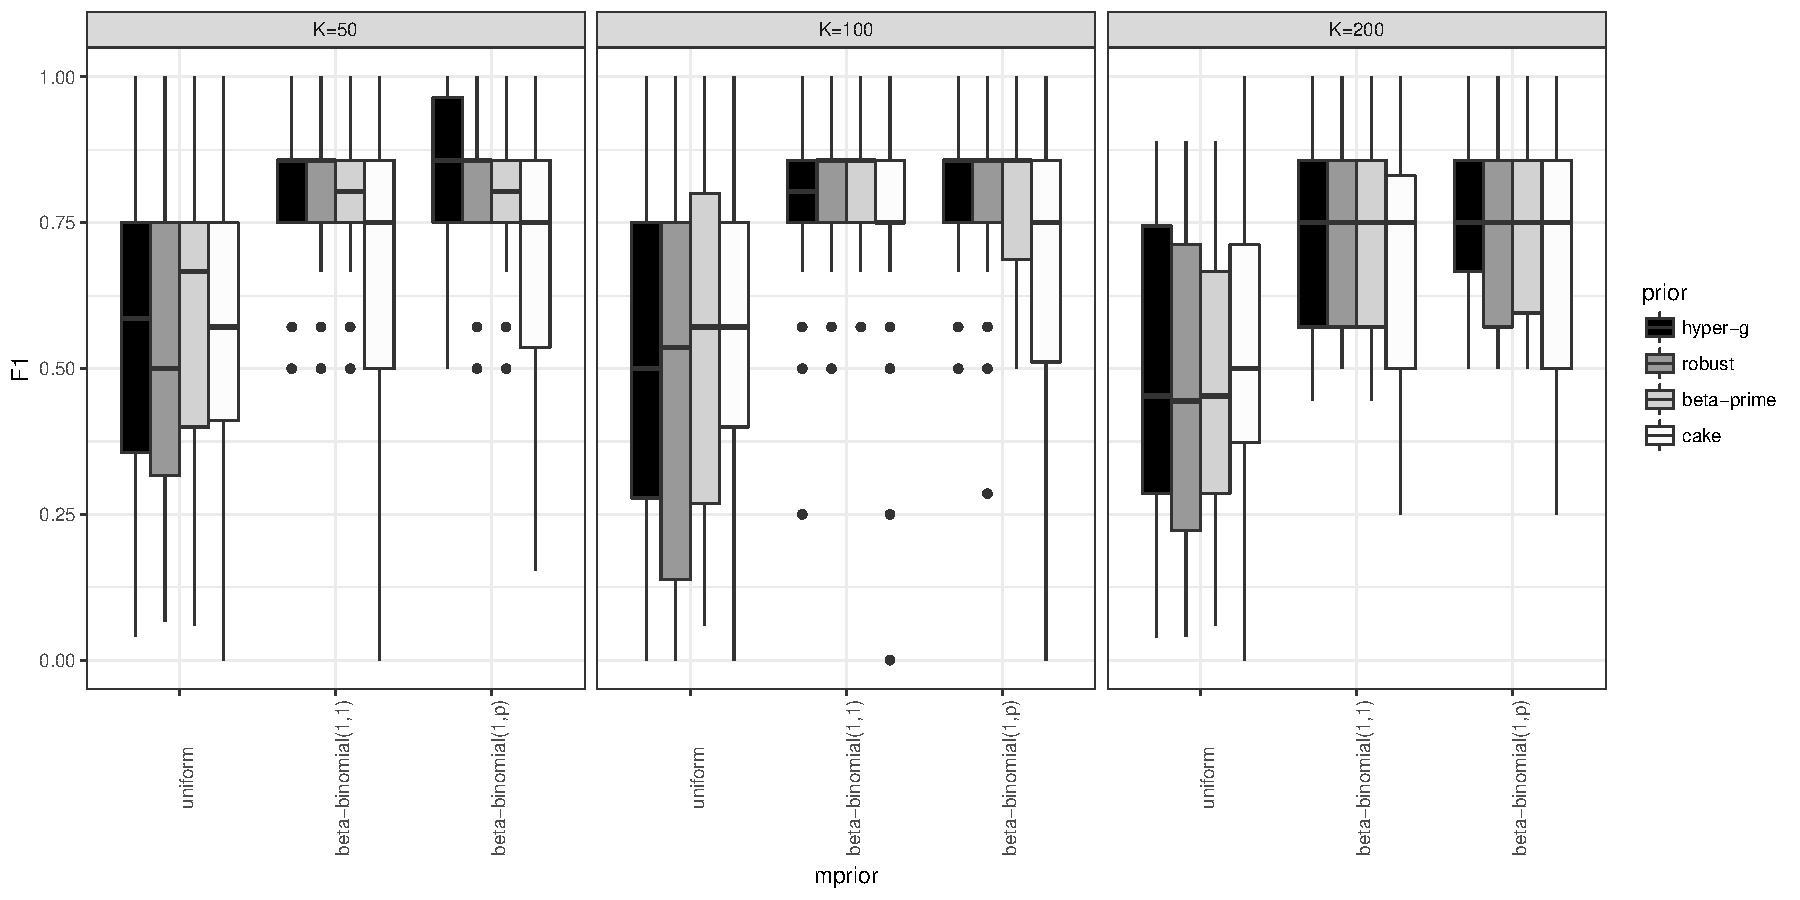
\includegraphics[width=0.95\textwidth]{./highDimPVA_F1.pdf}  
	\end{center}
	\caption{Comparison of the performance of the PVA method on the
						high-dimensional data set with different $g$ and $\vgamma$ priors using $F_1$ score.
						The hyper-$g$,
						robust Bayarri, Beta-prime and Cake priors on $g$ and the uniform, beta-binomial(1, 1) and beta-binomial(1, p) priors on $\vgamma$ are used.}
	\label{fig:cva_posterior_models}
\end{figure}

\begin{figure}[h!]
	\begin{center}	
		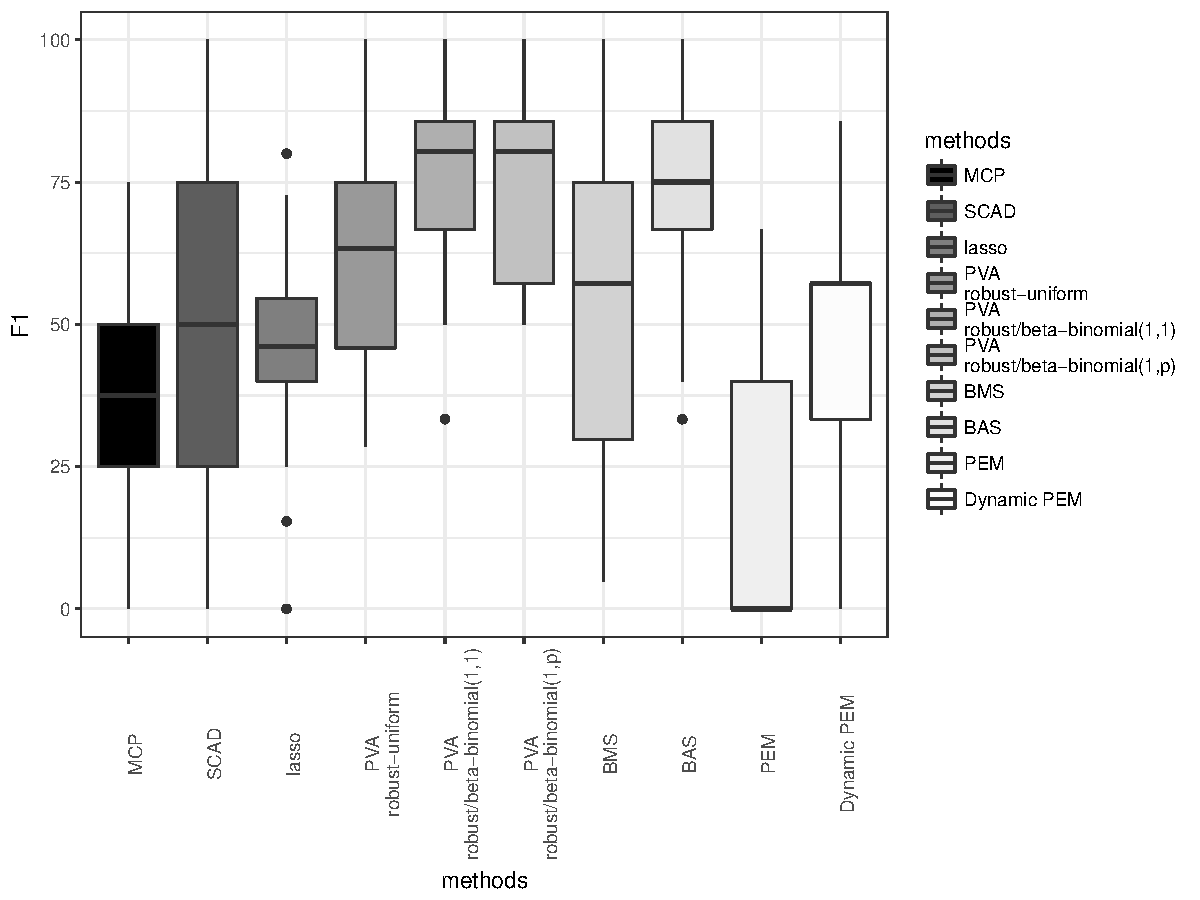
\includegraphics[width=0.95\textwidth]{./highDimPVA_F1_compare.pdf}  
	\end{center}
	\caption{Comparison of the performance of the MCP, SCAD, lasso, PVA, BMS, BAS and PEM methods on the
						high-dimensional data set using $F_1$ score. For PVA, the
						robust Bayarri prior on $g$ and the uniform, beta-binomial(1, 1) and beta-binomial(1, p) priors
						on $\vgamma$ are used.}
	\label{fig:cva_posterior_models}
\end{figure}

\subsubsection{Exploration of the posterior model space}

If the covariates in a model selection problem are highly collinear then the posterior distribution will be
highly multi-modal when a spike-and-slab prior structure is used. This can make seeking the optimal model very
challenging, due to the many local optima. In this section, we present a series of numerical experiments which
demonstrate the capability of our algorithm to successfully find the models with high posterior probability in
such situations.

Our population of bit strings $\mGamma^{(0)} = (\vgamma_1^{(0)}, \ldots, \vgamma_K^{(0)})$ with
$K = 20$ particles was randomly initialised from a sequencial of independent Bernoulli trials with probability
of success $1/2$.
Figure \ref{fig:cva_posterior_models1} shows all $4,096$ posterior model probabilities ordered by the model's
bit strings, represented by blue dots. Superimposed over this are the models found by CVA, represented by
red dots.
We can clearly see a few peaks in the full posterior distribution. Our experiment aims to show
that most of these posterior peaks are successfully identified by our algorithm.

% We begin by using the setting $\lambda = 1$, allowing particle repulsion between each of the models within the
% population.

\begin{figure}	
	\includegraphics[width=0.95 \textwidth]{code/blma/cva_low_dimensional.pdf}
	\caption{Posterior model probabilities when $p = 12$. Red points denote models visited by the CVA
						algorithm, while blue points are models that were not visited. Note that the CVA algorithm
						visits the highest posterior probability points first}
	\label{fig:cva_posterior_models1}
\end{figure}

\subsection{Communities and crime dataset}
\label{sec:crime}

We use the {\tt Communities and Crime} dataset obtained from the
UCI Machine Learning Repository   \\

\url{http://archive.ics.uci.edu/ml/datasets/Communities+and+Crime}  \\

\noindent 
The data collected was part
of a study by \cite{Redmond2002} combining socio-economic data
from the 1990 United States Census, law enforcement data from the 1990 United States Law Enforcement Management and Administrative
Statistics
survey, and crime data from the 1995 Federal Bureau of Investigation's Uniform
Crime Reports.

The raw data consists of 2215 samples of 147 variables the first 5 of which
we regard as non-predictive, the next 124 are regarded as potential
covariates while the last 18 variables are regarded as potential response
variables. Roughly 15\% of the data is missing. We proceed with a complete
case analysis of the data.
We first remove any potential covariates which contained missing values leaving
101 covariates. We also remove the variables {\tt rentLowQ} and
{\tt medGrossRent} since these variables appeared to be nearly linear
combinations of the remaining variables (the matrix $\mX$ had two singular
values approximately $10^{-9}$ when these variables were included).  We use the
{\tt nonViolPerPop} variable as the response. We then remove any remaining
samples where the response is missing. The remaining dataset consist of 2118
samples and 99 covariates. Finally, the response and covariates are standardized to have mean 0 and standard deviation 1. Empirical correlations between variables range from $3.3\times10^{-5}$ to $0.999$.

\begin{figure}
	\begin{center}	
		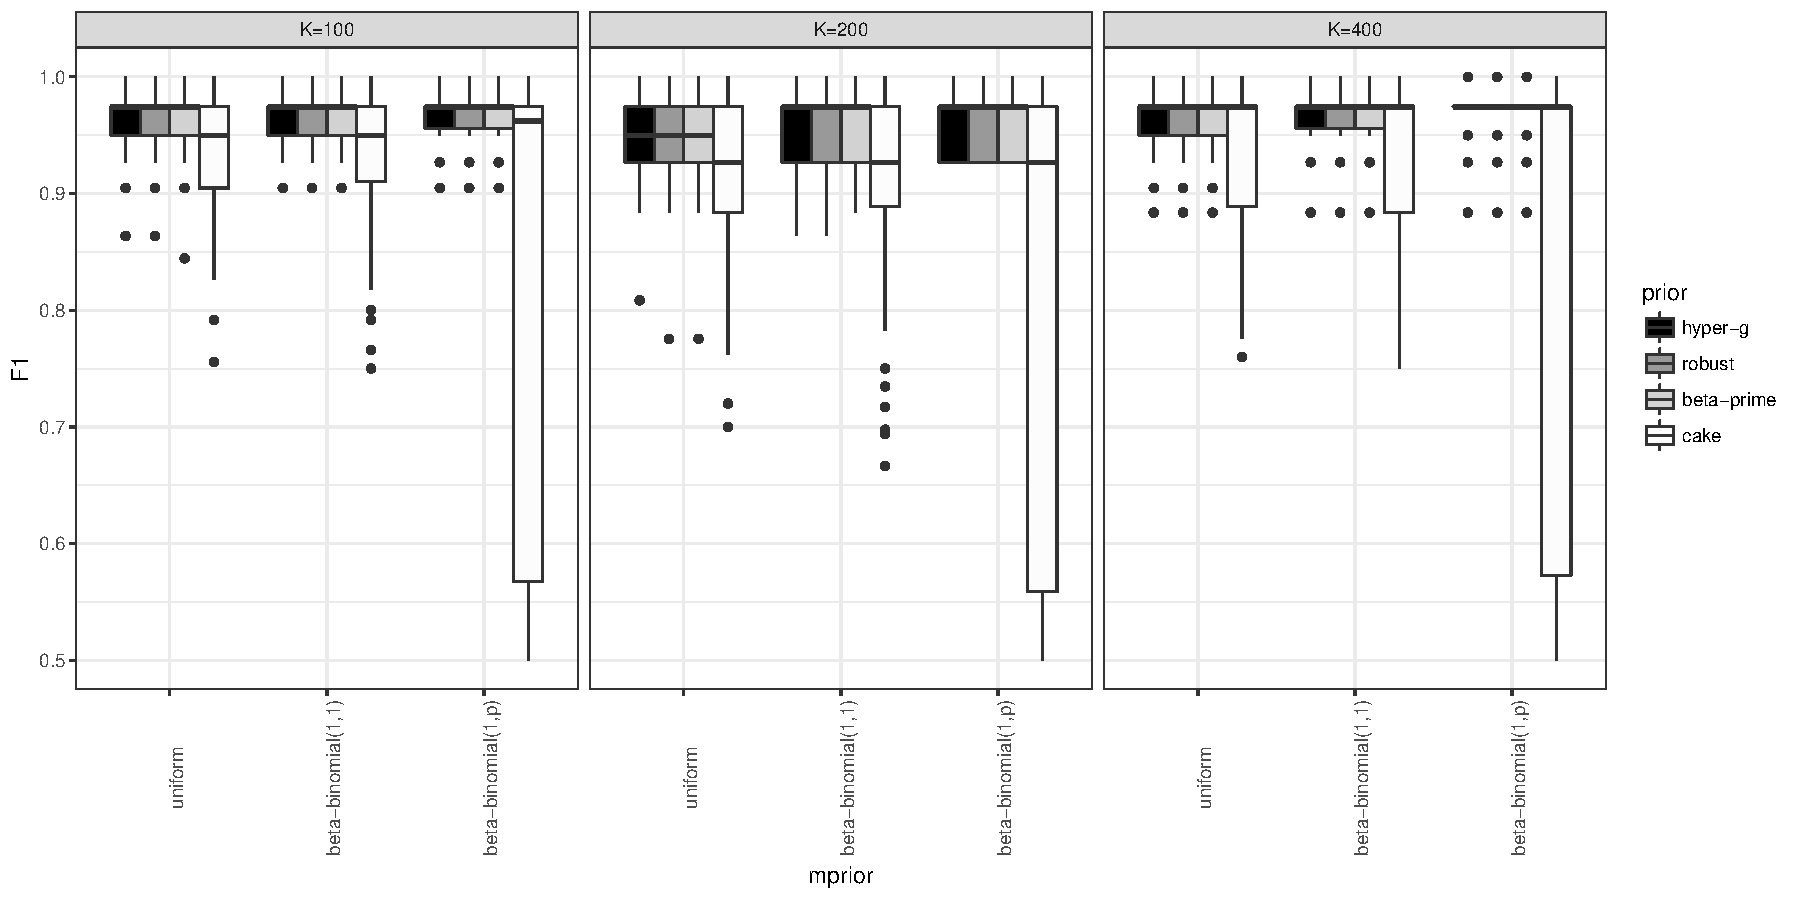
\includegraphics[width=0.95\textwidth]{./commPVA_F1.pdf}  
	\end{center}
	\caption{Comparison of the performance of the PVA method on the
						Communities and Crime data set with different $g$ and $\vgamma$ priors using $F_1$ score.
						The hyper-$g$,
						robust Bayarri, Beta-prime and Cake priors on $g$ and the uniform, beta-binomial(1, 1) and beta-binomial(1, p) priors on $\vgamma$ are used.}
\end{figure}

\begin{figure}
	\begin{center}	
		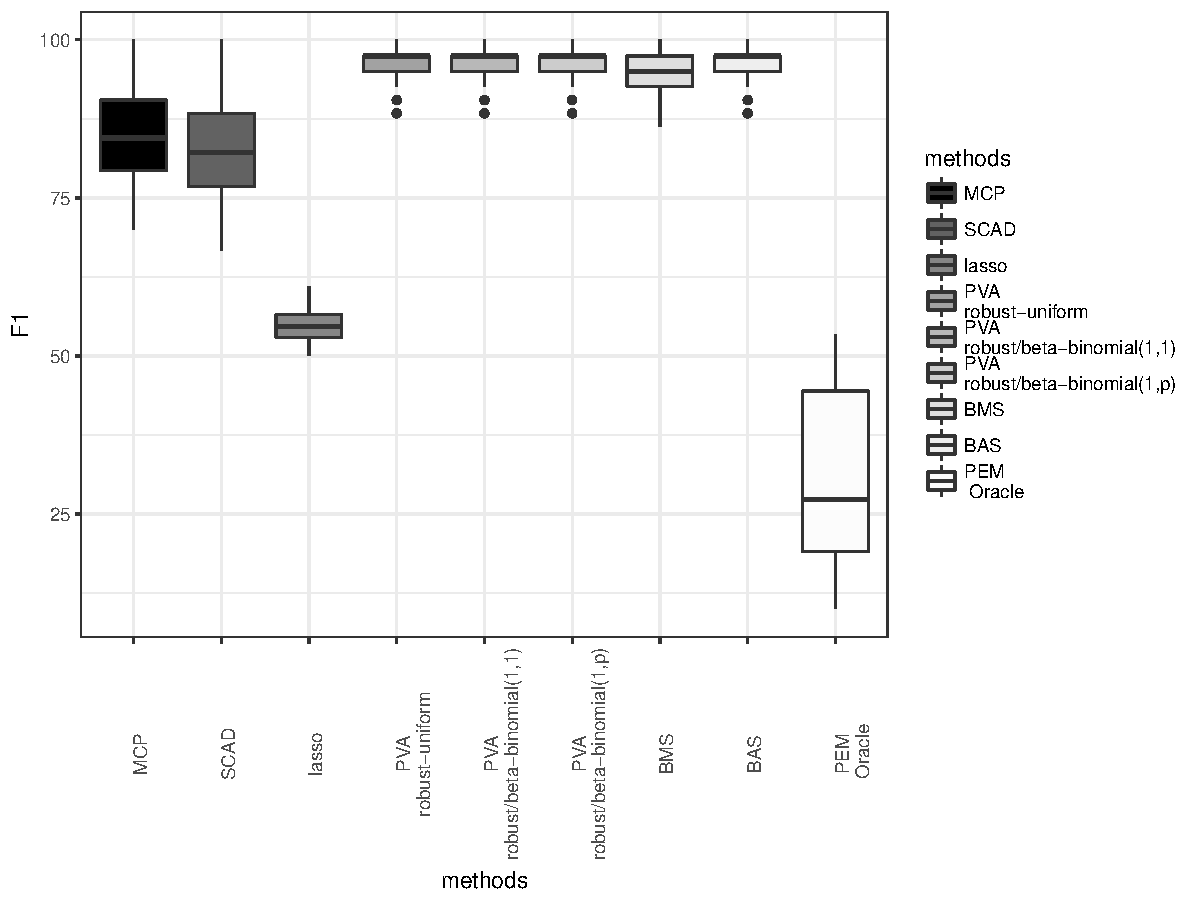
\includegraphics[width=0.95\textwidth]{./commPVA_F1_compare.pdf}  
	\end{center}
	\caption{Comparison of the performance of the MCP, SCAD, lasso, PVA, BMS, BAS and PEM methods on the
						Communities and Crime data set using $F_1$ score. For PVA, the
						robust Bayarri prior on $g$ and the uniform, beta-binomial(1, 1) and beta-binomial(1, p) priors
						on $\vgamma$ are used.}
\end{figure}

\subsection{Quantitative trait loci dataset}
\label{sec:QTL}

	For our final $p>n$ simulation example we will use the design matrix based on an
experiment on a backcross population of $n=600$ individuals for a single large 
chromosome of 1800 cM. This giant chromosome was covered by 121 evenly 
spaced markers from \cite{Xu2007}. Nine of the markers overlapped with QTL ofthe main effects 
and 13 out of the ${121 \choose 2} = 7260$ possible marker pairs had interaction 
effects. The $\mX$ matrix combines the main effects and interaction effects to
make a $600\times 7381$ matrix. The values of the true coefficients are listed in 
Table 1 of \cite{Xu2007} ranging from 0.77 to 4.77 in absolute magnitude and
correlations range from 0 to 0.8 where most of the higher correlation occurs
along the off-diagonal values of the correlation matrix of the covariates. Here
we center the $\mX$ matrix and simulate new data from $\vy = \mX\vbeta_0 + \vvarepsilon$
where $\vvarepsilon = (\varepsilon_1,\ldots,\varepsilon_n)^\top$ and the $\vvarepsilon_i$
are independently drawn with $\vvarepsilon_i \sim N(0,20)$. Similar simulation
studies were conducted in \cite{Xu2007} and \cite{LiSillanpaa2012}. This
process was repeated $50$ times and the results are summarized in Figure \ref{fig:04}.
For this simulation setting VB has the best model selection accuracy,
smallest MSEs and smallest parameter biases of all the methods compared.
The Lasso, SCAD, MCP, EMVS, VB and BMS methods took 1.5, 1.5, 1.8, 1229, 2011, 5327
seconds respectively.

\begin{figure}[h!]
	\begin{center}	
		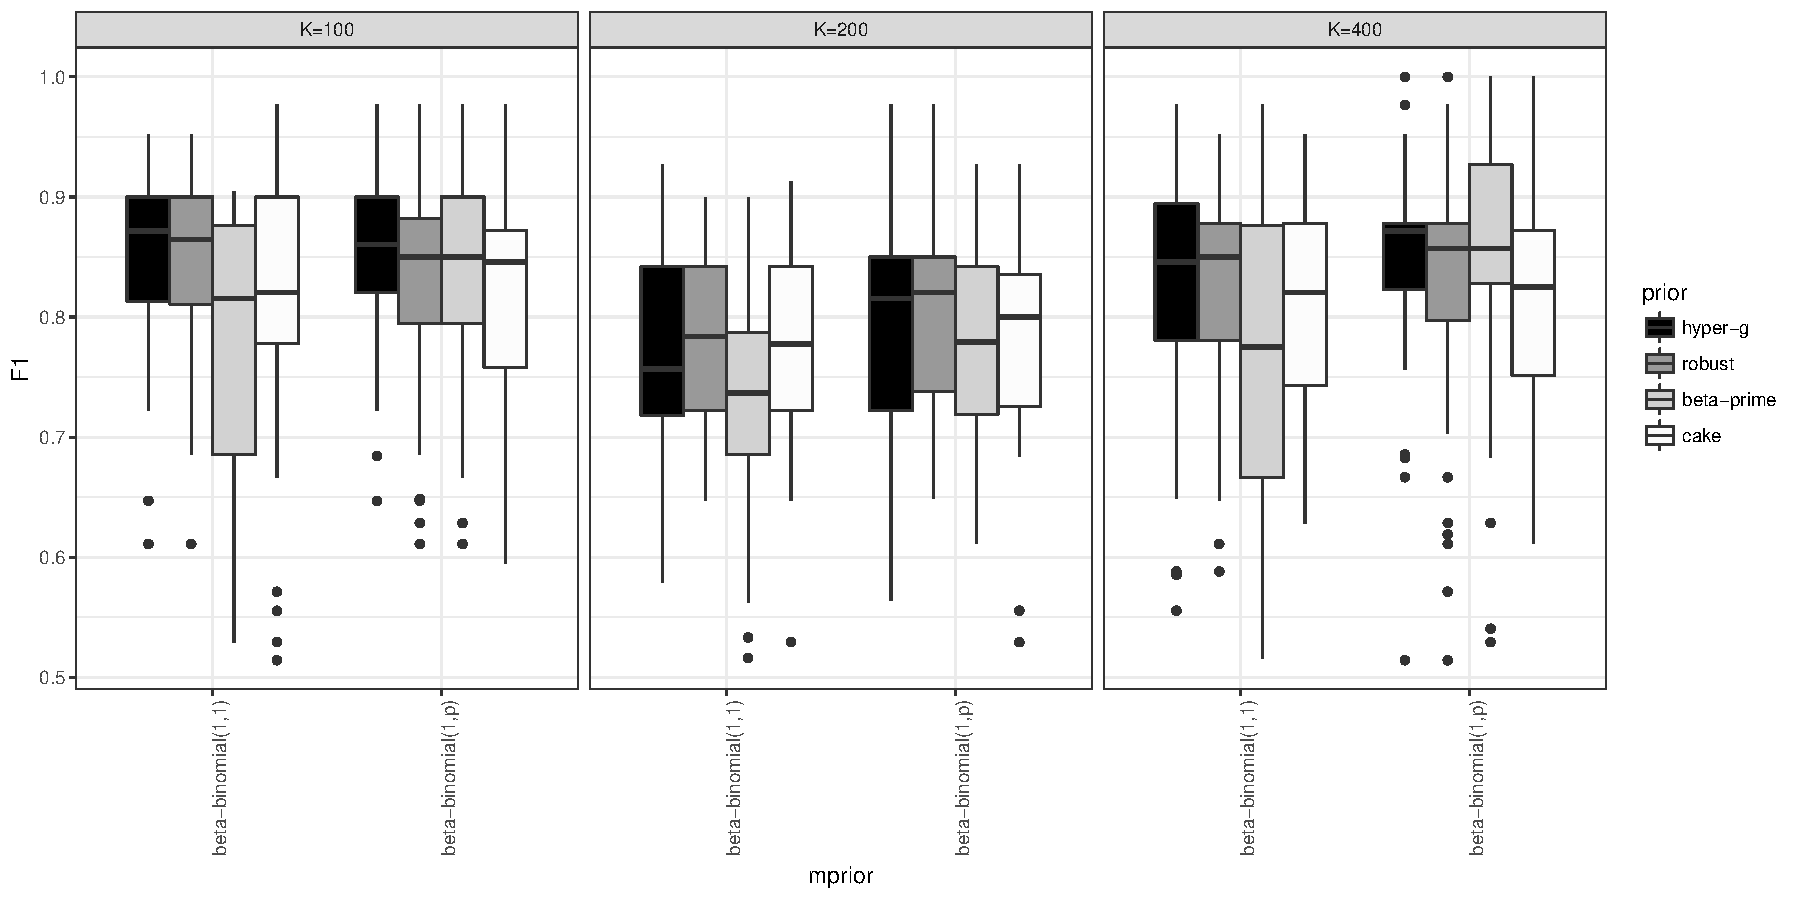
\includegraphics[width=0.95\textwidth]{./qtlPVA_F1.pdf}  
	\end{center}
	\caption{Comparison of the performance of the PVA method on the
						QTL data set with different $g$ and $\vgamma$ priors using $F_1$ score.
						The hyper-$g$,
						robust Bayarri, Beta-prime and Cake priors on $g$ and the uniform, beta-binomial(1, 1) and beta-binomial(1, p) priors on $\vgamma$ are used.}
\end{figure}

\begin{figure}[h!]
	\begin{center}	
		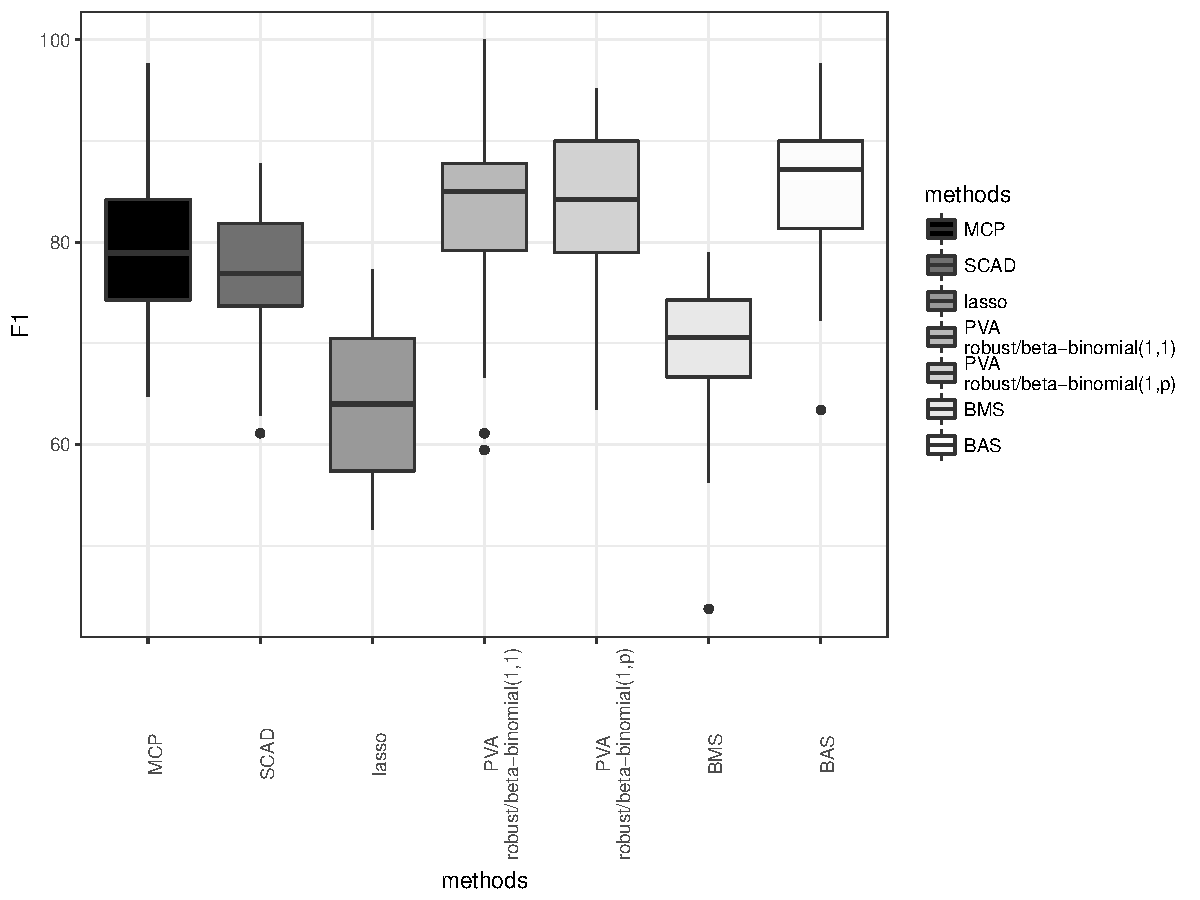
\includegraphics[width=0.95\textwidth]{./qtlPVA_F1_compare.pdf}  
	\end{center}
	\caption{Comparison of the performance of the MCP, SCAD, lasso, PVA, BMS, BAS and PEM methods on the
						QTL data set using $F_1$ score. For PVA, the
						robust Bayarri prior on $g$ and the uniform, beta-binomial(1, 1) and beta-binomial(1, p) priors
						on $\vgamma$ are used.}
\end{figure}


% Mine
\subsection{$n < p$, High dimensional example, Particle EM}

We first present an example where $n > p$ and $p$ is relatively small ($p = 12$), to allow for the full
enumeration of the model space. Later, we show an example for the important $p > n$ case. We compare our
results  against the Lasso (\cite{Tibshirani1996}), SCAD (\cite{Fan2001}), MCP (\cite{Zhang2010}), {\tt BMS}
(\cite{Zeugner2015}) and {\tt VARBVS} (\cite{Carbonetto2012}) algorithms.


\subsection{$p > n$}

% \begin{table}
% 	\caption{Simulation results including the average number of modes located, the average percentage of
% 	posterior coverage achieved, and the percentage of times that the global mode was located, for various
% 	population sizes $(K=20, 50, 100)$ and choices of repulsion $\lambda=0, 1, 2, 3$}
% 	\label{tab:result2}
% 	\begin{tabular}{l|llll|llll|llll|llll}
% 	\hline
% 	 					& \multicolumn{4}{c}{K=20} 	& \multicolumn{4}{c}{K=50} & \multicolumn{4}{c}{K=100} \\
% 	$\lambda$ & 0 & 1 & 2 & 3 & 0 & 1 & 2 & 3 & 0 & 1 & 2 & 3 & 0 & 1 & 2 & 3 \\
% 	\hline
% 	\# Modes & \\
% 	\% Posterior & 83.1 & 84.7 & 83.7 & 82.3 & 84.7 & 83.2 & 85.4 & 84.8 & 81.9 & 82.9 & 83.9 & 84.6 & 83.9 & 81.5 & 82.0 & 85.2 \\
% 	\% Global Mode & 91 & 90 & 87 & 82 & 86 & 85 & 80 & 90 & 90 & 90 & 86 & 91 & 88 & 91 & 76 & 88 \\
% 	\hline
% 	\end{tabular}

% \end{table}

% Show posterior probabilities on the log scale
As Figure \ref{fig:cva_posterior_models} shows, 
in the plots of the log posterior probabilities of the models, the particles can be seen clustering at the
highest probability models first, then spreading through the medium and low probability models. From these
plots we can see that once $K$ is high enough, there is a good variety of high, medium and low posterior
probability models in the population of particles. The coverage of the posterior probability distribution
by the population of particles is high, as the particles tend to cluster towards the higher posterior
probability models as CVA's greedy search algorithm proceeds.

\subsection{Comparison of CVA against other model selection methods on simulated data sets}

	% TP <- sum(vgamma.hat[pos])
	% TN <- sum(1 - vgamma.hat[neg])
	% FP <- sum(vgamma.hat[neg])
	% FN <- sum(1 - vgamma.hat[pos])
	
	% sensitivity <- TP/length(pos)
	% specificity <- TN/length(neg)
	% precision <- TP/sum(vgamma.hat)
	% recall <- TP/(TP + FN)
	% accuracy <- (TP + TN)/(TP + TN + FP + FN)
		
	% F1 <- 2*precision*recall/(precision+recall)		

The method used to assess the quality of the variable selection was to generate data from a known true model
$\vgamma$, and then compare this against the model $\widehat{\vgamma}$ found by each of the model selection
methods that we  compared. We then calculated the $F_1$ score for $\widehat{\vgamma}$.

% ,

% where
% $$F_1 = 2 \times \text{precision} \times \text{recall} / (\text{precision} + \text{recall})$$ with
% $\text{precision} = \text{true positives} / (\text{true positives} + \text{false positives})$ and
% $\text{recall} = \text{true positives} / (\text{true positives} + \text{false negatives})$.

% When running CVA,
% three methods of initialising $\Gamma$ were tried.
% A cold start where each $\gamma_{ij}$ in $\gamma_i$, $1 \leq i \leq K$ was initialised randomly from a
% $\text{Bernoulli}(p)$ distribution, with $p = 10 / |\vgamma|$.

% Two methods of warm start were also tried, to explore whether the CVA algorithm could do better by being
% initialised from another method than by being initialised randomly: 
% a warm start from SCAD where models with more covariates were preferred, and
% a warm start from SCAD where models with higher likelihood were preferred.

The experiments were repeated with 
the Cake prior, Maruyama's Beta-prime prior, Liang's hyper-g prior and Bayarri's robust prior.
The results of the algorithm were found to be insensitive to the choice of prior.
For each combination of population size, data set, and prior the experiment was repeated 50 times.

\subsubsection{High-dimensional example $p > n$, Quantitative Trait Locus}
The Quantitative Trait Locus (QTL) example is taken from \cite{Xu2007}. A BC population of $n=600$ was
simulated for a single large chromosome of $1800$ cM. This chromosome was covered by 121 evenly spaced
markers. Nine of the markers overlapped with QTL of the main effects and 13 out of the $\binom{121} 2 = 7,260$
possible marker pairs had interaction effects.

The CVA method was compared against Lasso, SCAD, Mcp, BMS and VARBVS. The {\tt BMS} method was run with
$1,000,000$ iterations. While the $F_1$ scores from this method were excellent, the runtimes of the BMS method
with this number of iterations were prohibively long - from 10 minutes to half an hour. When the number of
iterations was reduced to $100,000$ less, the resulting $F_1$ scores were much poorer. The {\tt VARBVS} method
was run with $\sigma = 10.0$ and $sa = 10.0$, which improved the $F_1$ score obtained.

When initialising $\Gamma$ with a warm start from SCAD preferring models with more covariates or with higher
likelihood, CVA performed poorly with a lower number of particles (K=$20$). Performance improved as the number
of particles in the population was increased, as can be seen in Figures \ref{fig:QTL_warm_start_covariates}
and \ref{fig:QTL_warm_start_likelihood}. Performance was better when $\Gamma$ was initialised randomly, for
all population sizes $K=20$, $50$ or $100$.  CVA consistently achieved $F_1$ scores that were either
competitive with or higher than the competing methods that we examined. This indicates that the CVA algorithm
is sensitive to its' initialisation, and that as SCAD does poorly on these problems, CVA also does poorly
comparatively with a warm start from SCAD, although still better than SCAD alone.

% \begin{figure}
% \includegraphics[width=0.95 \textwidth]{QTL_covariates_maruyama.pdf}
% \label{fig:QTL_warm_start_covariates}
% \caption{$F_1$ scores for CVA on the simulated QTL data with $\Gamma$ initialised from the SCAD models, with
% models with more covariates preferred. Here $K=20$, $50$ and $100$ respectively}
% \includegraphics[scale=0.33]{code/QTL/results/20_generate_data_QTL_warm_start_covariates_log_prob1.pdf}
% \includegraphics[scale=0.33]{code/QTL/results/50_generate_data_QTL_warm_start_covariates_log_prob1.pdf}
% \includegraphics[scale=0.33]{code/QTL/results/100_generate_data_QTL_warm_start_covariates_log_prob1.pdf}
% \end{figure}

% \begin{figure}
% \includegraphics[width=0.95 \textwidth]{QTL_likelihood_maruyama.pdf}
% \label{fig:QTL_warm_start_likelihood}
% \caption{$F_1$ scores for CVA on the simulated QTL data with $\Gamma$ initialised from the SCAD models, with
% models with higher likelihood preferred. Here $K=20$, $50$ and $100$ respectively}
% \end{figure}


Initialising $\Gamma$ randomly, CVA performed poorly by comparison with either of the warm start methods
above, as can be seen from Figure \ref{fig:QTL_cold_start}.
% \begin{figure}
% \includegraphics[width=0.95 \textwidth]{QTL_cold_maruyama.pdf}
% \label{fig:QTL_cold_start}
% \caption{$F_1$ scores for CVA on the simulated QTL data with $\Gamma$ initialised randomly.
% 					Here $K=20$, $50$ and $100$ respectively}
% \includegraphics[scale=0.33]{code/QTL/results/20_generate_data_QTL_cold_start_log_prob1.pdf}
% \includegraphics[scale=0.33]{code/QTL/results/50_generate_data_QTL_cold_start_log_prob1.pdf}
% \includegraphics[scale=0.33]{code/QTL/results/100_generate_data_QTL_cold_start_log_prob1.pdf}
% \end{figure}

When initialising $\Gamma$ with a warm start from SCAD preferring models with higher likelihood,
CVA performed less well on the QTL example than SCAD preferring models with more covariates, but still
better than other competing methods except for MCP,
as can be seen from Figure \ref{fig:QTL_warm_start_likelihood}

\section{Variable inclusion for small data sets}

We compared variable selection using CVA against exact variable selection on five small data sets,
Hitters, Bodyfat, Wage, College and US Crime. 
The variable inclusion probabilities were estimated by taking the sum of the columns of the population
of models selected $\mGamma$
weighted by marginal likelihood of each model.
The exact variable inclusion probabilities were calculated by summing the columns of the matrix of all possible
models $\mGamma$ weighted by marginal likelihood of each model.
The mean relative error of the variable inclusion probabilities estimated by CVA was calculated,
and the results of these comparisons are presented in Table \ref{tab:variable_inclusion_rel_error}.
The number of particles in the population $K$ affected the
variable inclusion probability in the variables selected by CVA, while the marginal probability
$p(\vgamma | \vy)$ used to weight models in $\Gamma$ seemed to have only a very minor impact.
% Is this still true?
When the robust Bayarri prior is chosen to rank models in CVA,
the marginal probability $p(\vgamma | \vy)$ changes a lot as opposed to ranking models with other priors.
From the previous section, we see that changing the CVA model ranking
marginal had a large impact on the $F_1$ score obtained.
Variables with low posterior probability are truncated to 0, as CVA seeks higher posterior probability models,
ignoring the lower posterior probability models.

\begin{table}
\begin{tabular}{|ll|rrr|rrr|}
	\hline
	Dataset & Prior & & $<=0.5$ & & & $>0.5$ &\\
	& & $K = 20$ & $K = 50$ & $K = 100$ & $K = 20$ & $K = 50$ & $K = 100$ \\
	\hline
	Bodyfat&BIC&$0.63$&$0.48$&$0.37$&$0.07$&$0.01$&$0.02$\\
	&g$.$safe&$0.66$&$0.52$&$0.42$&$0.07$&$0.01$&$0.02$\\
	&Robust&$0.65$&$0.52$&$0.4$&$0.07$&$0.01$&$0.02$\\
	&ZE&$0.65$&$0.51$&$0.39$&$0.06$&$0.01$&$0.02$\\
	College&BIC&$0.7$&$0.58$&$0.49$&$0.03$&$0.02$&$0.03$\\
	&g$.$safe&$0.9$&$0.78$&$0.64$&$0.06$&$0.06$&$0.06$\\
	&Robust&$0.88$&$0.78$&$0.63$&$0.06$&$0.06$&$0.06$\\
	&ZE&$0.82$&$0.66$&$0.57$&$0.03$&$0.06$&$0.06$\\
	Hitters&BIC&$0.74$&$0.64$&$0.5$&$0.12$&$0.07$&$0.06$\\
	&g$.$safe&NA&$0.81$&$0.83$&NA&$0.17$&$0.07$\\
	&Robust&$0.84$&$0.81$&$0.75$&$0.29$&$0.17$&$0.07$\\
	&ZE&$0.79$&$0.72$&$0.67$&$0.27$&$0.13$&$0.05$\\
	USCrime&BIC&$0.82$&$0.7$&$0.64$&$0.47$&$0.15$&$0.12$\\
	&g$.$safe&$0.76$&$0.71$&$0.64$&$0.45$&$0.16$&$0.12$\\
	&Robust&$0.79$&$0.7$&$0.61$&$0.35$&$0.14$&$0.08$\\
	&ZE&$0.76$&$0.7$&$0.64$&$0.45$&$0.16$&$0.13$\\
	Wage&BIC&$0.67$&$0.49$&$0.35$&$0$&$0$&$0$\\
	&g$.$safe&$0.69$&$0.47$&$0.33$&$0$&$0$&$0$\\
	&Robust&$0.69$&$0.47$&$0.32$&$0$&$0$&$0$\\
	&ZE&$0.69$&$0.47$&$0.32$&$0$&$0$&$0$\\
	\hline
\end{tabular}
\label{tab:variable_inclusion_rel_error}
\caption{Relative error of the variable inclusion probability estimated by CVA to the
					exact variable inclusion probability, partitioned by exact probability under or equal to $0.5$ and
					over $0.5$}
\end{table}

% Small data set, Kakadu
\begin{figure}[h!]
	% \includegraphics[scale=0.5]{posterior_prob_Kakadu.pdf}
	% \includegraphics[scale=0.5]{inclusion_error_Kakadu.pdf}

	\caption{CVA was run on the Kakadu data set. The total posterior model probability and error in posterior 
						variable inclusion probability were calculated using the exact posterior model and variable  
						inclusion probability from every possible sub-model. These were calculated for a range of 
						population sizes from 25 to 500, in 25 model increments.
						As the population increases, the total posterior model probability increases while the error in 
						posterior variable inclusion probabliity decreases.}
\end{figure}

% VietNam
% GradRate
% UScrime

% Interpretation of results
The same general trends were observed in all small data sets. Total posterior probability is higher for the
beta- binomial model prior than for the uniform model prior, while the variable inclusion error is lower. This
same general trend is seen regardless of g-prior. Total posterior probability increases with increased
population size $K$, while variable inclusion error decreases. Although the CVA algorithm is deterministic,
variation in the results amongst the trials is seen due to the random initialisation of $\mGamma$.
